
\section{Introduction}

GPS devices are widely used in orchard planting and maintenance. This location-based system allows orchardist to check trajectory of tractors. 

Usually, GPS units record more data than necessary, and causes more errors due to the shelter from branches. 

Local simplification algorithms. This algorithm focuses on a couple of particular consecutive points. By analyzing the relationship among these points, a decision is made that which point can be deleted or retained. Distance threshold algorithm is one of these algorithms. All points, for which the distance to the preceding track point is less than a predetermined threshold is deleted. Direction changing algorithm is another one. The point is retained if the change in direction is greater than a predetermined threshold  \cite{ivanov2012real}. 

Global simplification algorithms. These algorithms have an overview of all tracked points. After analyzing the relationships among these points, a decision will be made about which one or more points to delete or retain. The Douglas-Peucker algorithm is one of them \cite{douglas1973algorithms}.

It is apparently that global simplification algorithms can be used on off-line data analyses and local simplification algorithms will perform better on on-line or real-time track simplification. 

However, a pertinent algorithm is required in our case. 

\section{Preliminary}
In this section, we elaborate an algorithm used in simplifying global trajectories. 

Trajectory is a connection by a time series successive positions recorded by GPS devices. A classical GPS device records skeleton information, including time stamp, latitude, longitude, number of available satellites, etc. Recently, researchers try to enrich trajectory (called Semantic Trajectory) by adding background geographic information to discover meaningful pattern \cite{ying2011semantic}. A TS simplification method, represented in \cite{chen2009trajectory}, consider both the skeleton information and semantic meanings of a trajectory when performing simplification.

In our case, a GPS log is a sequence time series GPS points $p_i \in P$, $P=\{ p_1,p_2, \cdots, p_n \}$. Each GPS point $p_i$ contains information of time stamp, latitude and longitude, and semantic information of velocity, heading direction and boom status, which can be written in form of
\begin{equation}
T=\{p_t=[x_t,y_t,v_t,\theta_t,b_t] | t \in \mathbb{R} \}.
\end{equation}
Sequentially connect these points will give us a tractor trajectory.

For a  tractor working on an orchard, there are two status of a boom, working and not working. These information is recorded by GPS units, and using $b=1$ to represented for working and $b=0$ for not working.

$\mathbf{Segment}$ A segment is a part of consecutive trajectory. Regarding to the status of boom, trajectory can be simply divided into two kinds of segment in our dataset, one is boom-working, the other is boom-not-working. 

$\mathbf{Direction}$. Direction $\theta$ denotes the heading direction of a tractor at a specific point location. This parameter uses north direction as a basis, in which way $\ang{0} \leq \theta < \ang{360}$.

\section{Track Simplification Algorithm}

The first two steps are initial simplification to reduce some errors caused by mis-operation and GPS units bugs.
\begin{itemize}
\item Step 1. Merging. If the length of a segment composed by consecutive boom working or not-working points is less than a threshold, merge this one into its backward segment. 
\item Step 2. Remove time stamp duplicated data.
\end{itemize}
Now only two types of segment points are left in GPS log, boom working and not-working, and the length of each segment is greater than the predetermined threshold.

The following algorithm is based on the relationship between a candidate point $p_i$ and it's neighboring points $p_{i-1}$ and $p_{i+1}$, and the importance of the $p_i$ in the segment where it belongs to. 

\begin{itemize}
\item Rule 1. The candidate point $p_i$ is retained if it is not linear predictable or cannot be used for linear predicting. With the velocity information $v_{i-1}, v_i$ at point $p_{i-1}, p_i$ and time differences $\Delta t_{i-1} = |t_{i}-t_{i-1}|,\Delta t_{i} = |t_{i+1}-t_{i}|$, an estimated position can be calculated by $\hat{p}_i=\Delta t_{i-1} p_{i-1}$, $\hat{p}_{i+1}=\Delta t_{i} p_{i}$. If the distance $|\hat{p}_i-p_i|$ or $|\hat{p}_{i+1}-p_{i+1}|$ is less than a threshold, then the point $p_i$ is not linear predictable or cannot be used for linear predicting.

\item Rule 2. Select a candidate point $p_i$. Retain this point if the distance between $p_i$ and $p_{i-1}$ is greater than the threshold $d$, where $d$ is the mean distances of these points $p_{i-1}, p_i, \cdots, p_{i+k}$ with same boom status $b_{i-1}=b_i=\cdots=b_{i+k}$. 

\item Rule 3. Neighbor Heading Changing. The candidate point $p_i$ belongs to the track if $|\theta_i-\theta_{i-1}| + |\theta_i-\theta_{i+1}|>\theta$, where $|\theta_i-\theta_{i-1}|$ and $ |\theta_i-\theta_{i+1}|$ are the direction changes between points $p_i$ and $p_{i-1}$ and between points $p_i$ and $p_{i+1}$, $\theta$ is predefined threshold.

\item Rule 4. The candidate point $p_i$ belongs to the track if the boom status $b_i\neq b_{i-1}$.
\end{itemize}

Finally, the point $p_i$ belongs to the track if Rule 1 = TRUE or Rule 2 = TRUE or Rule 3 = TRUE or Rule 4 = TRUE.

\section{Evaluation}
Errors are measured by Synchronized Euclidean Distance \cite{lawson2011compression}. SED measures the distances between the original and compressed trace at the same time. As shown in figure 1\cite{lawson2011compression}. $P_{t1}, \cdots ,P_{t5}$ are original points. After simplification, the points $P_{t2}, P_{t3}$ and $P_{t4}$ were removed. The black curve is the original trajectory, in contrast, gray dash line is the simplified trajectory. The gray point $P'_{t2}$ on simplified trajectory has the same time difference as the point $P_{t2}$ on original trajectory does. Then the distance between $P_{t2}$ and $P'_{t2}$ is calculated.


\begin{figure}[h]
\centering
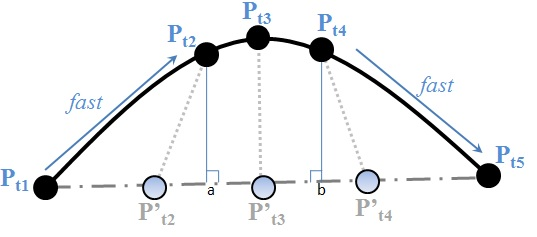
\includegraphics[width=16cm, height=8cm]{Chapters/06Spinoff/plot/sed.jpg}
\caption{Synchronized Euclidean Distance}
\end{figure}

Another way to calculate the difference between a GPS trace and its compressed version is to measure the perpendicular distance. This algorithms ignore the temporal component and use simple perpendicular distance. The figure 2 \cite{meratnia2004spatiotemporal} expresses these difference clearly. 

\begin{figure}[h]
\centering
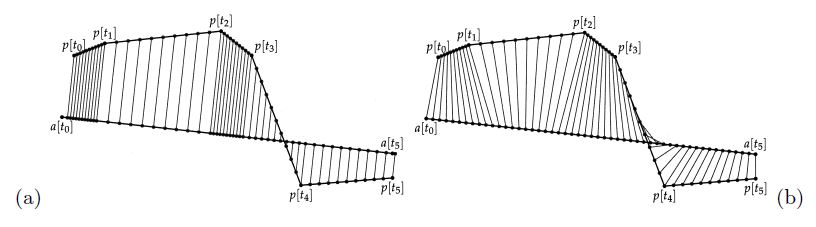
\includegraphics[width=13cm, height=5cm]{Chapters/06Spinoff/plot/ab.JPG}
\caption{(a) error measured at fixed sampling rate as sum of perpendicular distance chords; (b) error measured at fixed sampling rates as sum of time-synchronous distance chords.}
\end{figure}

\clearpage 

\section{Adaptive Kalman Filter}
Discrete Kalman Filter equations the describe the prediction step are
\begin{align*}
\hat{x}_k^-&=A\hat{x}_{k-1}+Bu_k \\
P_k^-&=AP_{k-1}A^\top+Q
\end{align*}
where $\hat{x}_k^-$ is a priori state estimate, $\hat{x}_k$ is a posteriori state estimate, $A$ is status transition matrix, $P_k^-$ is a priori estimate for error covariance, $u_k$ is an input parameter and $Q$ is process noise covariance. 

Discrete Kalman Filter equations the describe the correct step are
\begin{align*}
K_k&=P_k^-H^\top (HP_k^-H^\top+R)^{-1} \\
\hat{x}_k&=\hat{x}_k^-+K_k(z_k-H\hat{x}_k^-) \\
P_k&=(I-K_kH)P_k^-
\end{align*}
where $K_k$ is the Kalman gain matrix, $z_k$ is the observed data.

\section{Experimental  results}

Our original data set has 1021 rows, each of them contains latitude, longitude, velocity, heading direction and boom information. Douglas-Peucker Algorithm, with distance threshold $0.205m$, retained 847 points. Tractor Algorithm, given a predictable distance being $5m$ and heading direction changing being $\ang{30}$, returned the same amount of points. Under the same circumstance, we calculated SED and other information.

\begin{table}[h]
\centering
\caption{Error Comparing}
\label{tabledist}
\begin{tabular}{|l|l|l|l|}
\hline 
  & \textbf{Original Data} & \textbf{DP Algorithm} & \textbf{Tractor Algorithm}  \\
\hline 
\textbf{Number of Points} & 1021              & 847         & 847         \\
\textbf{Tracked Distances}(m)  & 74041.31     & 74038.33    & 74012.56     \\
\textbf{SED} (m)    & NA        & 1316.715    & 607.9587   \\
\hline 
\end{tabular}
\end{table}

Table (\ref{tabledist}) describe the results after simplifying with DP algorithm and Tractor Algorithm.

\begin{figure}
\centering
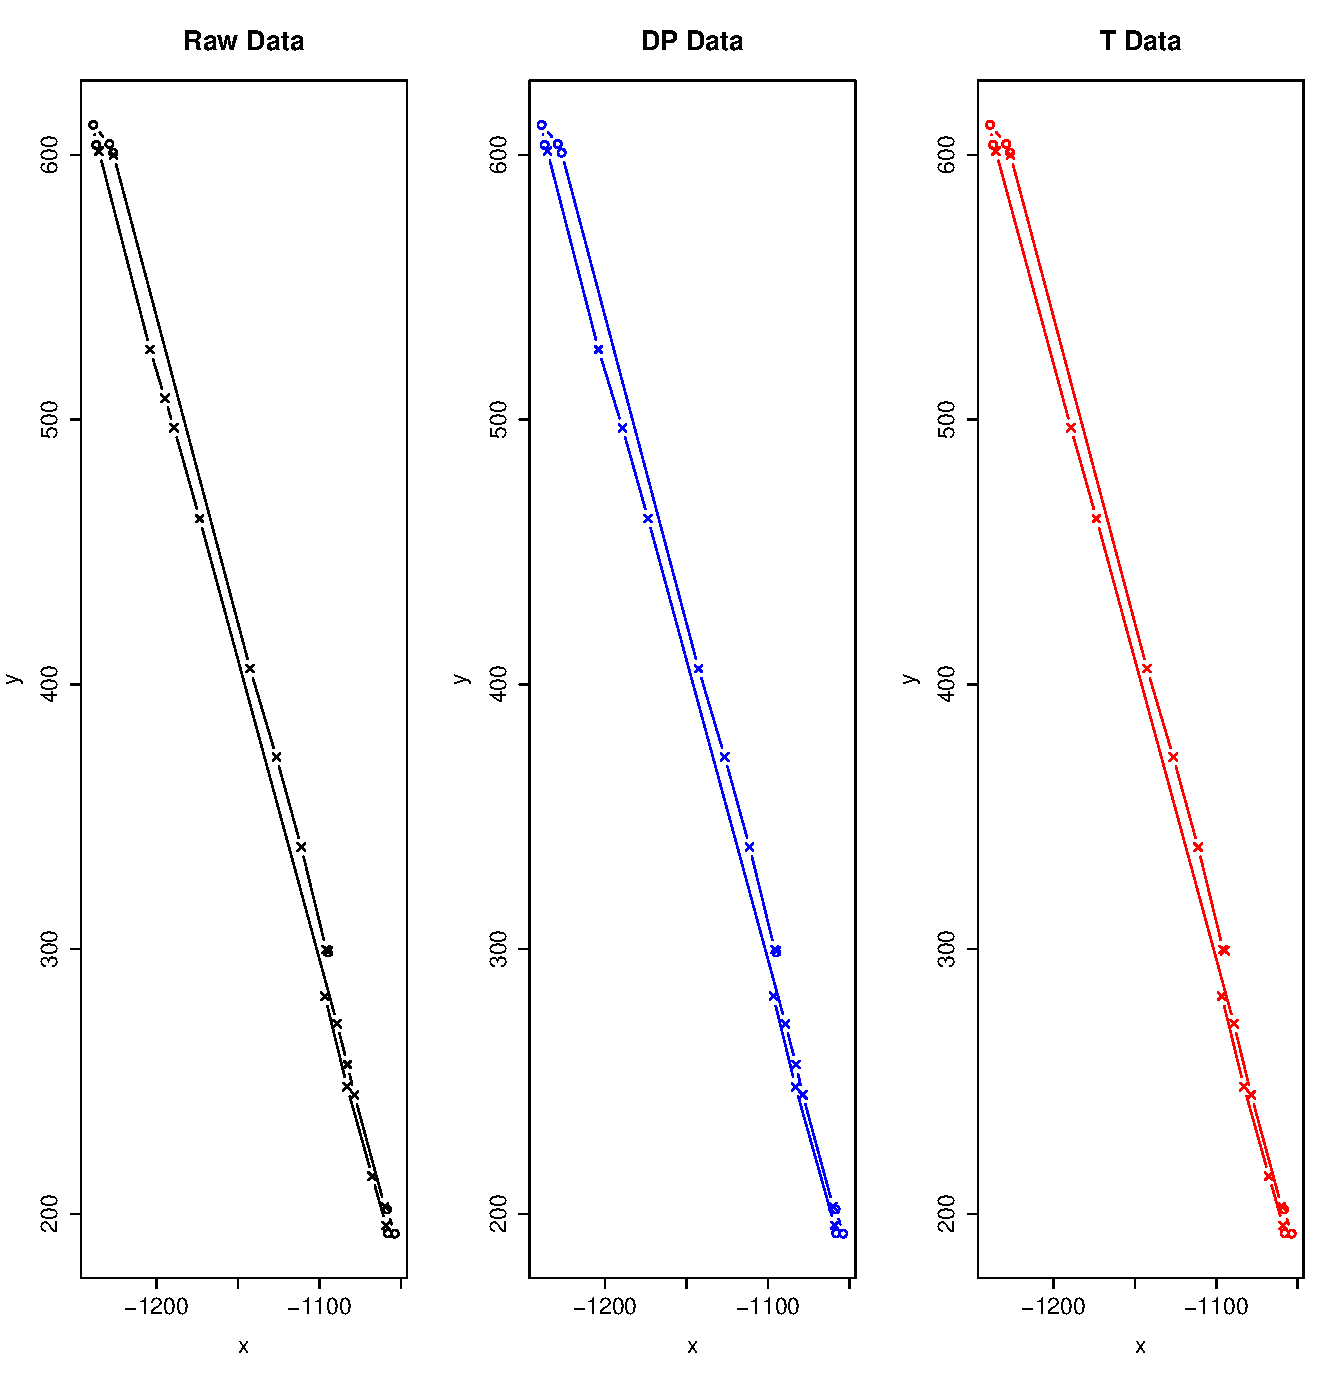
\includegraphics[width=15cm,height=8cm]{Chapters/06Spinoff/plot/3p1.pdf}
\caption{A segment start from time 2000 to 3000, recorded by GPS units. On the left side, it's the trajectory connected by raw data with 27 points. In the middle, it's the trajectory connected by simplified data with Douglas-Peucker Algorithm with 24 points. On the right side, it's the trajectory connected by simplified data with Tractor Simplification Algorithm with 23 points.}
\end{figure}

\begin{figure}
\centering
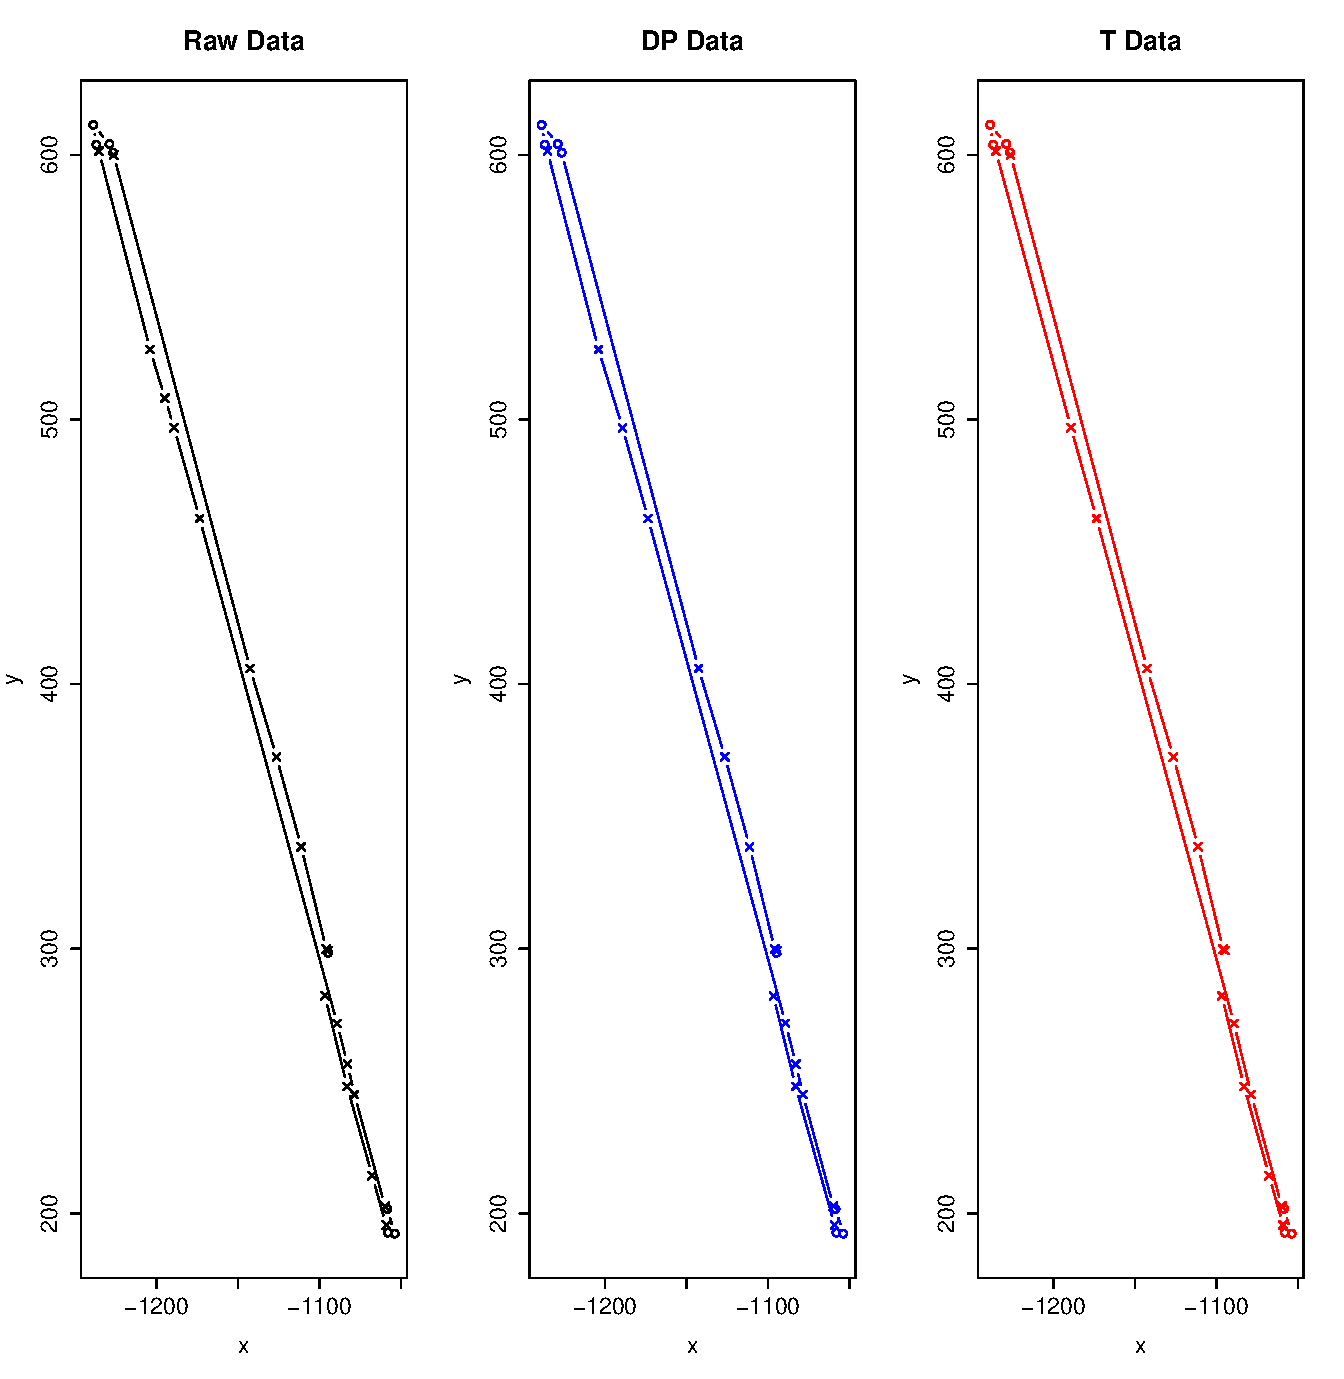
\includegraphics[width=15cm,height=8cm]{Chapters/06Spinoff/plot/km3p}
\caption{Trajectory fitted by Adaptive Kalman Filter. The errors of raw data, DP and tractor algorithm caused by AKF is  26.89217, 23.97877 and 23.97097 respectively.}
\end{figure}
